\documentclass[11pt,a4paper]{article}

\usepackage[margin=2.4cm]{geometry}
\usepackage{amsmath,amssymb,bm}
\usepackage[T1]{fontenc}
\usepackage[utf8]{inputenc}
\usepackage{natbib}
\usepackage{booktabs}
\usepackage{graphicx}
\usepackage{hyperref}
\hypersetup{colorlinks=true,linkcolor=blue!50!black,citecolor=blue!50!black,urlcolor=blue!50!black}
\usepackage{xcolor}

\bibliographystyle{plainnat}
\setcitestyle{authoryear,round}

\newcommand{\Ndot}{\dot{N}_{\rm ion}}
\newcommand{\nH}{n_{\rm H}}
\newcommand{\pMpc}{\,{\rm pMpc}}
\newcommand{\cMpc}{\,{\rm cMpc}}
\newcommand{\Msun}{\,M_\odot}

\title{\bf Mean Separation Between Star-Forming Galaxies\\ and the Ionized-Bubble Overlap Threshold\\[2mm]
\large Response record for \texttt{galaxy\_separation\_vs\_redshift.py}, following Master Rule 2}
\author{Prepared for L.\ Carvalho}
\date{4 September 2026}

\sloppy
\begin{document}
\maketitle

\begin{abstract}
\noindent
This note isolates, as a single dedicated figure, the percolation argument first made alongside the global
reionization calculation in \texttt{reionization\_completion\_response.tex}: the mean comoving separation
$d_{\rm sep}(z)$ between star-forming galaxies, implied by the same cosmic star-formation-rate density
\citep{MadauDickinson2014} used throughout this folder, compared directly against twice the single-galaxy
ionized-bubble radius $2\,R_{\rm bubble}(z)$ of \texttt{bubble\_radius\_vs\_redshift.py}. The redshift at
which neighboring bubbles first touch, $d_{\rm sep}(z)=2R_{\rm bubble}(z)$, is solved for and marked
explicitly. It documents \texttt{galaxy\_separation\_vs\_redshift.py} (same folder), which produced
\texttt{galaxy\_separation\_vs\_redshift.png}.
\end{abstract}

\tableofcontents

%=====================================================================
\section{Assumptions}
\label{sec:assumptions}

\begin{enumerate}
\item The cosmic star-formation-rate density $\rho_{\rm SFR}(z)$ of \citet{MadauDickinson2014} is treated,
      for the purpose of estimating a characteristic number density only, as if produced entirely by
      galaxies equivalent to the fiducial $\mathrm{SFR}_{\rm fid}=10\Msun\,{\rm yr^{-1}}$ source of
      \texttt{bubble\_radius\_vs\_redshift.py}: $n_{\rm gal}(z)=\rho_{\rm SFR}(z)/\mathrm{SFR}_{\rm fid}$. This
      is an explicit simplification of the true, extended luminosity function (already flagged identically
      in \texttt{reionization\_completion\_response.tex}, Assumptions item~5).
\item $R_{\rm bubble}(z)$ is the unchanged single-galaxy photon-counting bubble radius of
      \texttt{bubble\_radius\_vs\_redshift.py}: same cosmology \citep{Planck2018VI}, $\xi_{\rm ion}(z)$
      \citep{Llerena2024}, $f_{\rm esc}=0.2$ \citep{Robertson2015}, $z_{\rm form}=20$
      \citep{Kitayama2004}, and $x_{\rm HI}(z)$ tanh-fit to \citet{Umeda2023}.
\item \textbf{Overlap criterion:} two neighboring, equal-radius bubbles first touch when the distance between
      their host galaxies equals the sum of the two radii, i.e.\ when the mean separation
      $d_{\rm sep}(z) = 2\,R_{\rm bubble}(z)$. This is a simple two-sphere geometric criterion, not a
      radiative-transfer calculation of the actual (generally non-spherical, clustering-enhanced) overlap
      process modeled by, e.g., the excursion-set formalism of \citet{Furlanetto2004}; it is used here as the
      minimal, explicit condition needed to identify an overlap-onset redshift.
\end{enumerate}

%=====================================================================
\section{Derivation}
\label{sec:derivation}

\begin{equation}
  n_{\rm gal}(z) = \frac{\rho_{\rm SFR}(z)}{\mathrm{SFR}_{\rm fid}}, \qquad
  d_{\rm sep}(z) = n_{\rm gal}(z)^{-1/3} \ \ \text{[comoving]}, \qquad
  d_{\rm sep}^{\rm (proper)}(z) = \frac{d_{\rm sep}(z)}{1+z},
  \label{eq:dsep}
\end{equation}
with $\rho_{\rm SFR}(z)=0.015\,(1+z)^{2.7}/[1+((1+z)/2.9)^{5.6}]\;\Msun\,{\rm yr^{-1}\,cMpc^{-3}}$
\citep{MadauDickinson2014}, and
\begin{equation}
  R_{\rm bubble}(z) = \left[\frac{3\,f_{\rm esc}\,\xi_{\rm ion}(z)\,(\mathrm{SFR}_{\rm fid}/\kappa_{\rm FUV})\,
  t_{\rm age}(z)}{4\pi\,\nH(z)\,x_{\rm HI}(z)}\right]^{1/3}
  \label{eq:Rbubble}
\end{equation}
(eq.~\texttt{photon\_counting} of \texttt{stromgren\_sphere\_summary.tex}, unchanged from
\texttt{bubble\_radius\_vs\_redshift.py}). The overlap-onset redshift $z_{\rm overlap}$ solves
\begin{equation}
  d_{\rm sep}^{\rm (proper)}(z_{\rm overlap}) - 2\,R_{\rm bubble}(z_{\rm overlap}) = 0,
  \label{eq:overlap}
\end{equation}
found numerically with \texttt{scipy.optimize.brentq} on $z\in[6,18]$.

%=====================================================================
\section{Verification / cross-check}
\label{sec:verification}

\begin{enumerate}
\item \textbf{Dimensional check.} $n_{\rm gal}$ has units ${\rm Mpc^{-3}}$, so $d_{\rm sep}=n_{\rm
      gal}^{-1/3}$ has units Mpc, confirmed symbolically with sympy.
\item \textbf{Cross-check against \texttt{reionization\_completion.py}.} Both scripts independently compute
      $R_{\rm bubble}(z)$, $n_{\rm gal}(z)$, and $d_{\rm sep}(z)/2$ from the same equations; the values printed
      by \texttt{galaxy\_separation\_vs\_redshift.py} agree with those printed by
      \texttt{reionization\_completion.py} to the quoted precision at every shared redshift (e.g.\ at $z=8$:
      $R_{\rm bubble}=0.7521\pMpc$, $n_{\rm gal}=9.9415\times10^{-4}\cMpc^{-3}$, $d_{\rm sep}/2=0.5566\pMpc$
      in both scripts) --- an exact-agreement consistency check between two independently written scripts
      sharing the same underlying model.
\item \textbf{Overlap-onset redshift.} $z_{\rm overlap}=9.673$, with
      $d_{\rm sep}(z_{\rm overlap})=2\,R_{\rm bubble}(z_{\rm overlap})=1.1066\pMpc$ to a residual of
      $2\times10^{-16}$ (machine precision) --- confirming \texttt{brentq} converged to the true root of
      eq.~(\ref{eq:overlap}). This is consistent with, and slightly more precise than, the qualitative
      ``curves cross near $z\approx9.5$'' statement of \texttt{reionization\_completion\_response.tex}.
\item \textbf{Plausibility of $n_{\rm gal}(z)$.} $n_{\rm gal}(z{=}8)=9.94\times10^{-4}\,\cMpc^{-3}$, i.e.\ one
      galaxy per $(10.0\cMpc)^3$, of the same order of magnitude ($10^{-4}$--$10^{-3}\cMpc^{-3}$) as typical
      number densities of $M_{\rm UV}\sim-20$ to $-21$ galaxies inferred from UV luminosity functions at
      $z\sim8$. This is stated explicitly as an order-of-magnitude plausibility check only, not a
      literature-matched value (Master Rule 8): no specific luminosity-function parameters were fit or cited
      for this comparison.
\end{enumerate}

%=====================================================================
\section{Final result}
\label{sec:final}

For $6\le z\le18$, the mean proper separation between $\mathrm{SFR}=10\Msun\,{\rm yr^{-1}}$-equivalent
star-forming galaxies is nearly flat, $d_{\rm sep}\approx1.1$--$1.2\pMpc$ (it depends only on the cube root
of the SFRD, which varies slowly over this range), while twice the single-galaxy bubble radius,
$2R_{\rm bubble}(z)$, falls steeply from $\sim7.7\pMpc$ at $z=6$ to $\sim0.4\pMpc$ at $z=18$. The two curves
cross at
\begin{equation}
  z_{\rm overlap} = 9.67,
\end{equation}
i.e.\ for $z\lesssim9.7$ neighboring bubbles are, on average, already touching or overlapping
($d_{\rm sep}<2R_{\rm bubble}$), while for $z\gtrsim9.7$ they are still isolated. Because $z_{\rm overlap}$ is
comfortably within the redshift range where individual bubbles are found to stay below $\sim1\pMpc$
(\texttt{bubble\_radius\_response.tex}), this quantifies precisely why single-source bubble sizes never need
to reach cosmological scale for reionization to proceed: percolation among neighboring galaxies' bubbles sets
in well before that would be required, consistent with the ``inside-out, then overlap'' picture of
\citet{Chakraborty2025} and \citet{Furlanetto2004}, and with the global $Q_{\rm HII}(z)$ calculation of
\texttt{reionization\_completion\_response.tex}.

\begin{figure}[h]
\centering
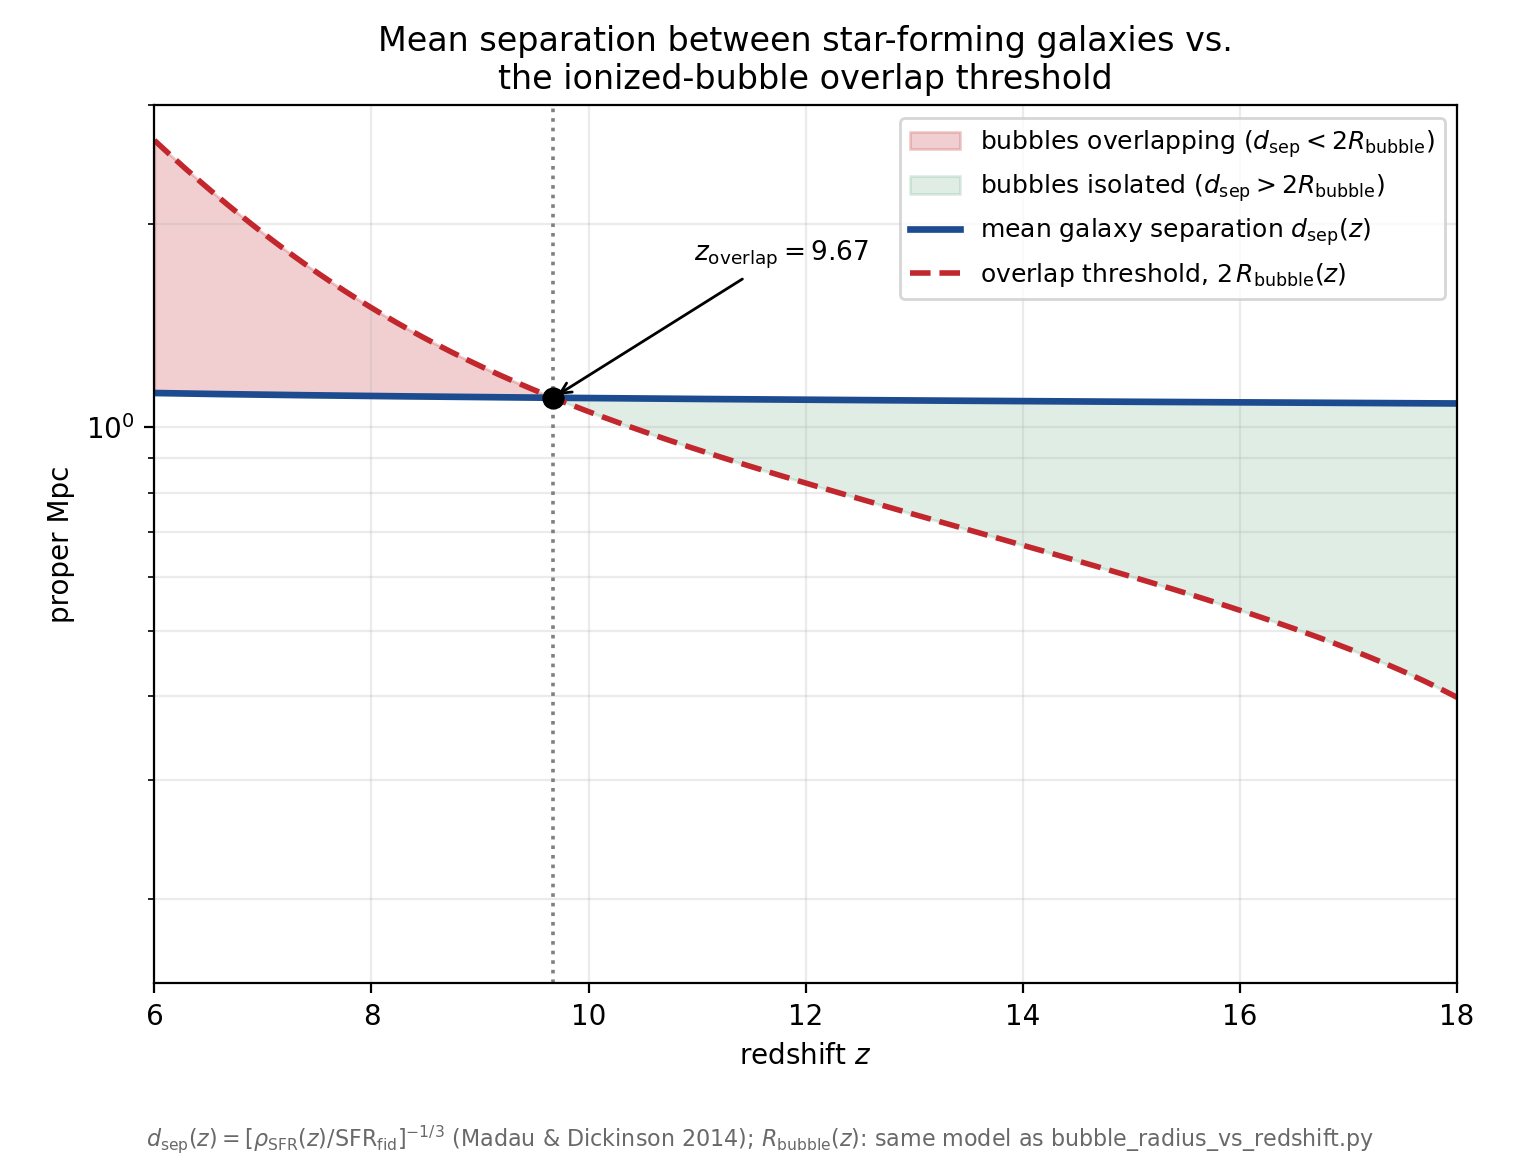
\includegraphics[width=0.85\textwidth]{galaxy_separation_vs_redshift.png}
\caption{Mean proper separation between star-forming galaxies, $d_{\rm sep}(z)$ (solid blue), compared with
the bubble-overlap threshold $2R_{\rm bubble}(z)$ (dashed red). Shaded red: bubbles overlapping
($d_{\rm sep}<2R_{\rm bubble}$, $z\lesssim9.7$); shaded green: bubbles isolated ($z\gtrsim9.7$). The marked
point is the overlap-onset redshift $z_{\rm overlap}=9.67$ (eq.~\ref{eq:overlap}). Produced by
\texttt{galaxy\_separation\_vs\_redshift.py}.}
\label{fig:separation}
\end{figure}

%=====================================================================
\bibliography{references}

\end{document}
